\section{Introduction}

The Santa Angélica intrusive complex (SAIC) is an elliptical elongated shape intrusion, which exposes an area of
approximately 200 km$^2$ emplaced in high-grade metamorphic (ortho and paragneisses, Figure~\ref{geology}a) country rocks \citep{Decampos2004}. The SAIC is also a representative example of the Southern portion of the Araçuaí Orogen post-collisional magmatism. It is characterized by the inversely zoned features, with granitic rocks located in its borders and mafic rocks occurring in two central cores (Figure~\ref{geology}b). The transition border-to-core is marked by a magma mixture zone with an intermediate composition \citep{Bayer1987, Schmidt1987}. This feature is interpreted as a bull's eye pattern, with concentric structured twin lobes separated by an internal shear zone \citep{Temporim2020}.

The study of the mechanisms responsible for the emplacement of post-collisional intrusions and the informational process of the country rocks might give important insights into the rheological condition of the crusts during the last stage of an orogen. For such, gravimetry can be applied in association with other techniques, such as anisotropy of magnetic susceptibility performed and micro-structural geology by \citet{Souza-Junior2021}. In this work, our goal is to reprocess the data acquired by the aforementioned authors to generate a residual Bouguer disturbance map for the SAIC rocks.


\begin{figure}[H]
  \centering
  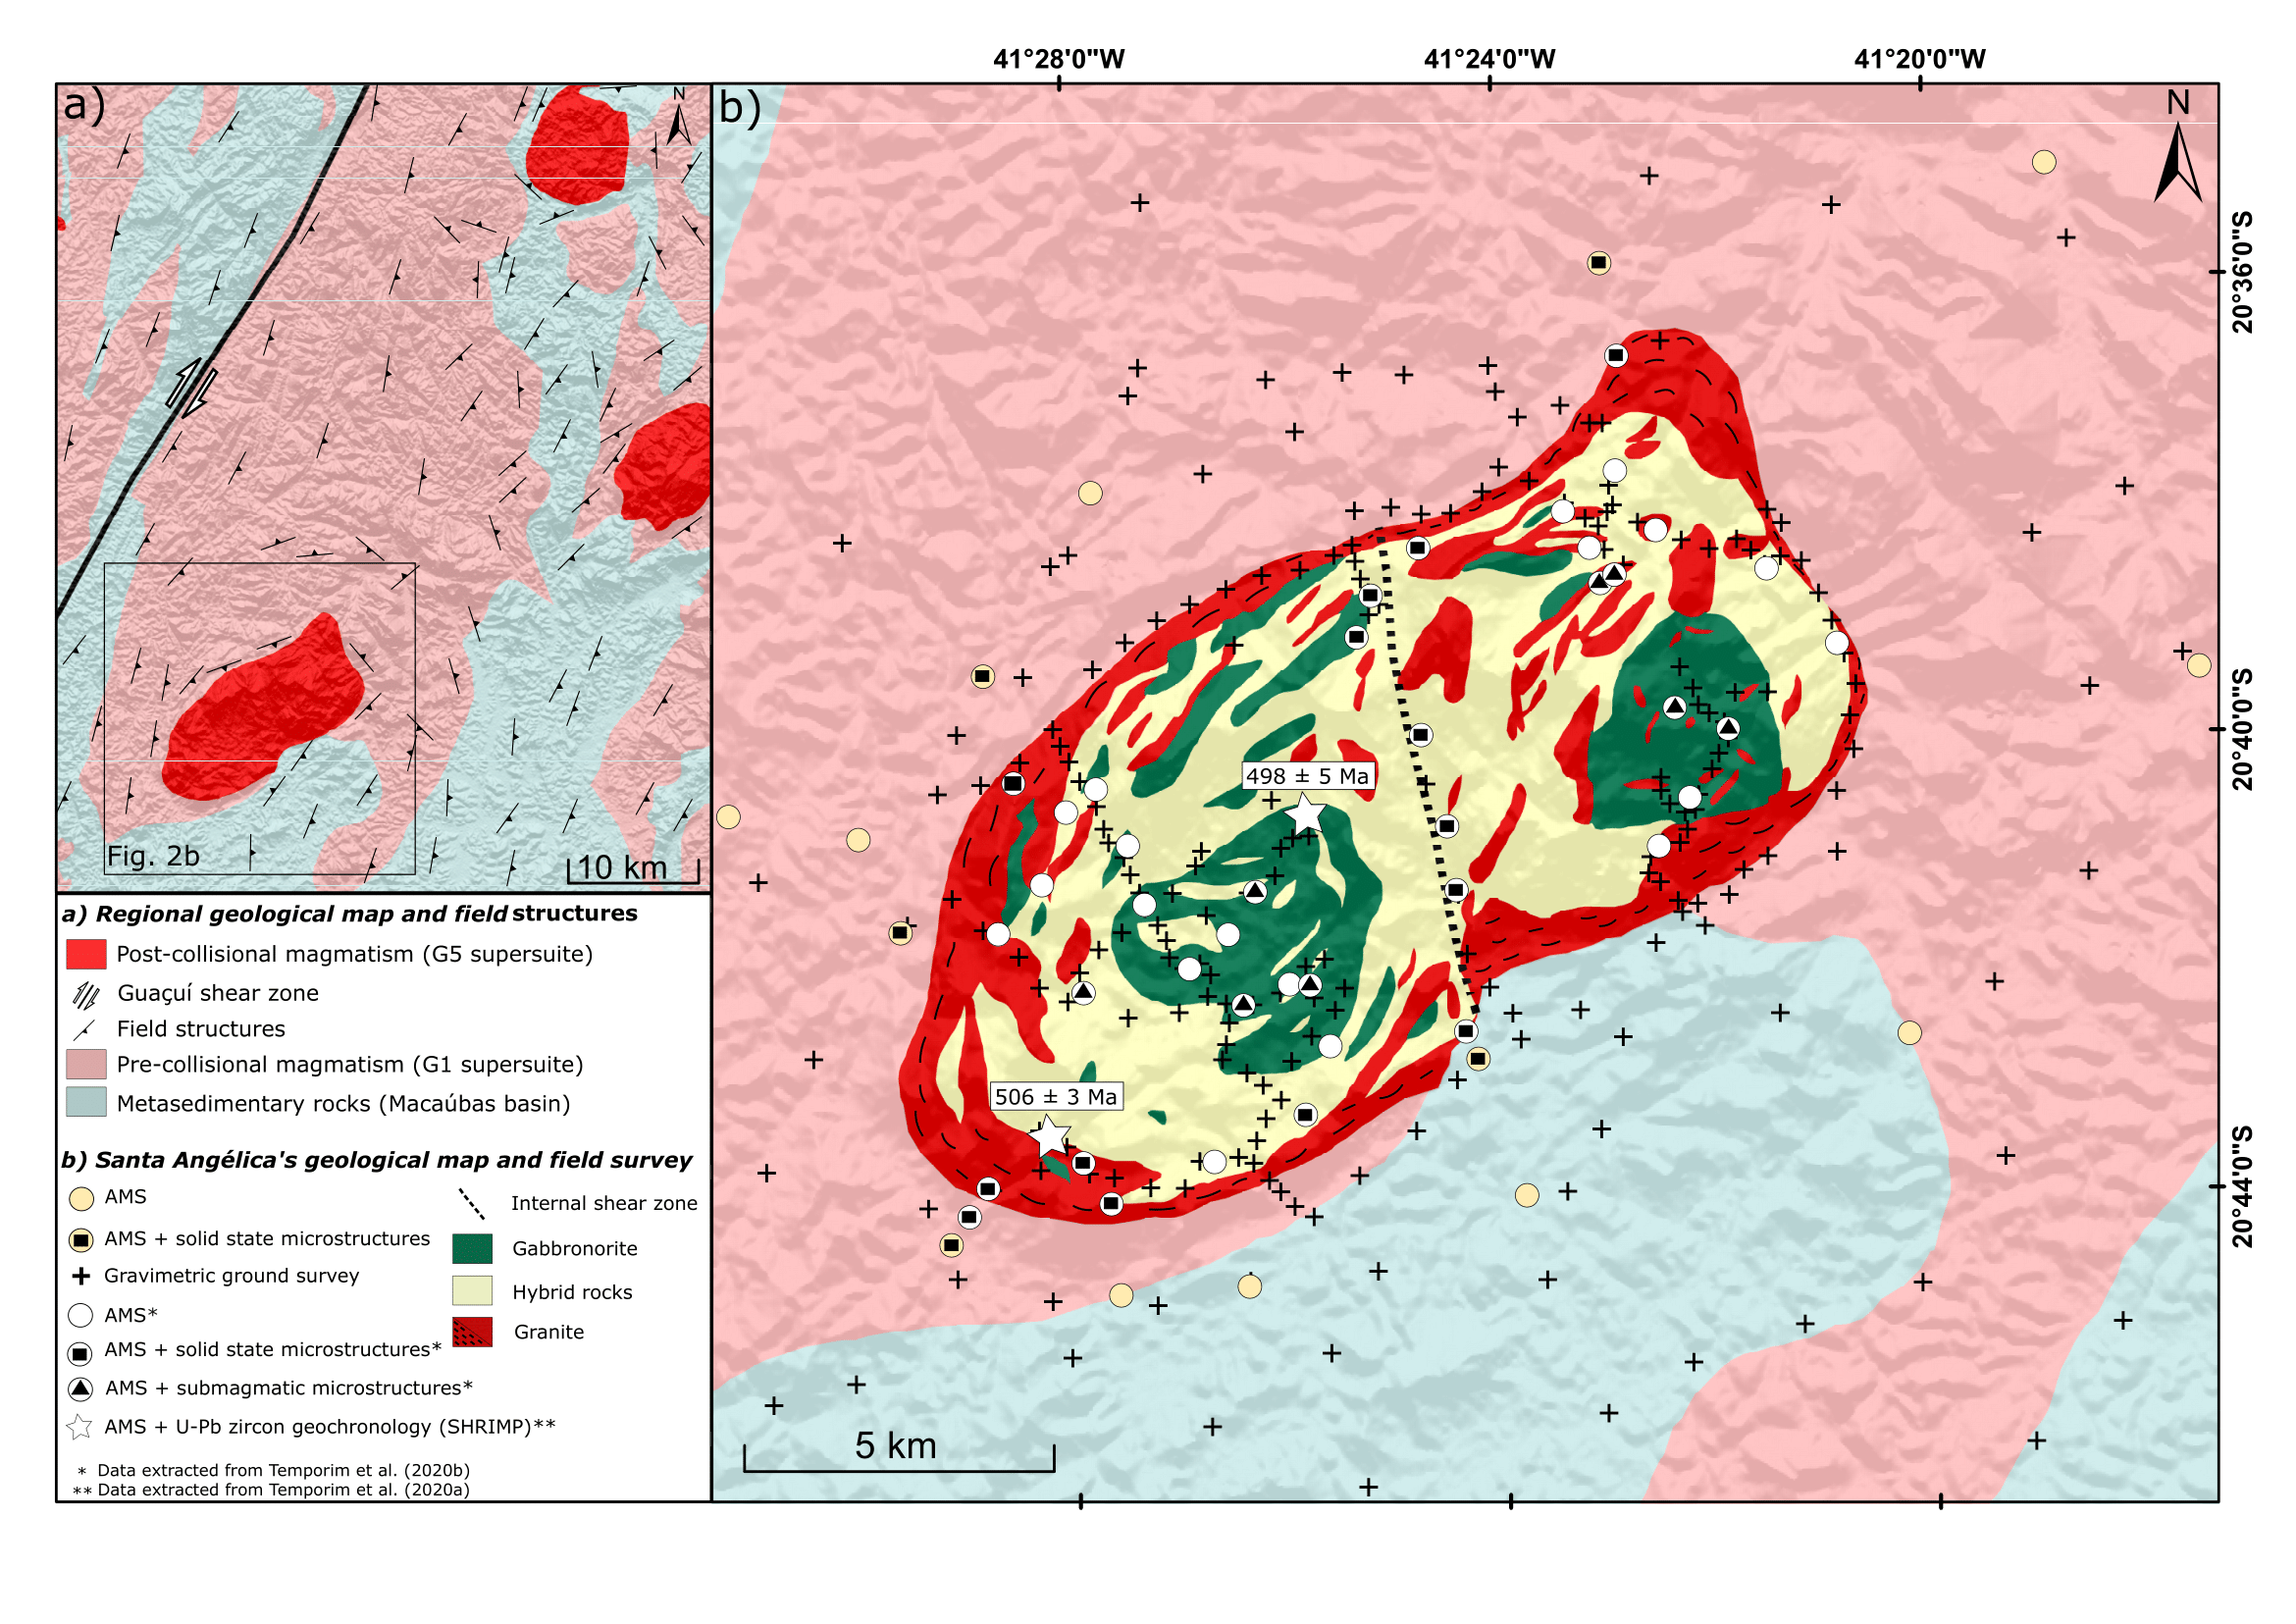
\includegraphics[width=1\linewidth]{figures/geology.png}
  \caption{
    Regional geological setting of the SAIC. a) SAIC's geological context within the country rocks and (b) its inversely zoned geological features. Extracted from \citet{Souza-Junior2021}.
      }
  \label{geology}
\end{figure}
